Clean Up is a turn-based dialogue game for two players focussed on cooperative strategy development and object rearrangement. Both players are presented with identical $7\times7$ ASCII-like grids, with a number of randomly distributed objects in the form of capital letters placed on them. Placement is different for each player and each player can only see their own grid, cf.~\cref{fig:clean_up_example}. The goal is to rearrange the objects in such away that their respective positions match across both grids. Scoring is based on the Euclidean distance of the identical objects on both grids.

Object rearrangement has been a long standing challenge in the field of artificial intelligence requiring understanding of the given situation, the action space, and spatial reasoning, cf.~\citet{DBLP:journals/corr/abs-2011-01975}, \citet{DBLP:journals/ral/ZengWYZDCD24}, \citet{DBLP:journals/access/KhanQCASR25}.

Collaborative reconstruction games, where one player knows the desired target state and has to instruct their counterpart to recreate it, have been extensively studied (see \citet{DBLP:journals/jair/SugliaKL24} for an overview). In this game, however, the players are on par and need to both negotiate their common goal state and a strategy of reaching it (cf.~\citet{DBLP:conf/sigdial/JeknicSK24}, which examines human-human and human-computer interaction in a similar game).

\begin{figure}[ht!]
    \centering
    % \newcounter{utterance}

\footnotesize  \setcounter{utterance}{1}
\setlength{\tabcolsep}{0pt}
\begin{supertabular}{c@{$\;$}|p{.15\linewidth}@{}p{.15\linewidth}p{.15\linewidth}p{.15\linewidth}p{.15\linewidth}p{.15\linewidth}}   
\# & $\;$A & \multicolumn{4}{c}{Game Master} & $\;\:$B\\
    \hline

\theutterance \stepcounter{utterance}  
    & & \multicolumn{4}{p{0.6\linewidth}}{
        \cellcolor[rgb]{0.9,0.9,0.9}{
            \makecell[{{p{\linewidth}}}]{
                \texttt{\tiny{[P1$\langle$GM]}}
                {<GAME DESCRIPTION>}\\
                \centering
                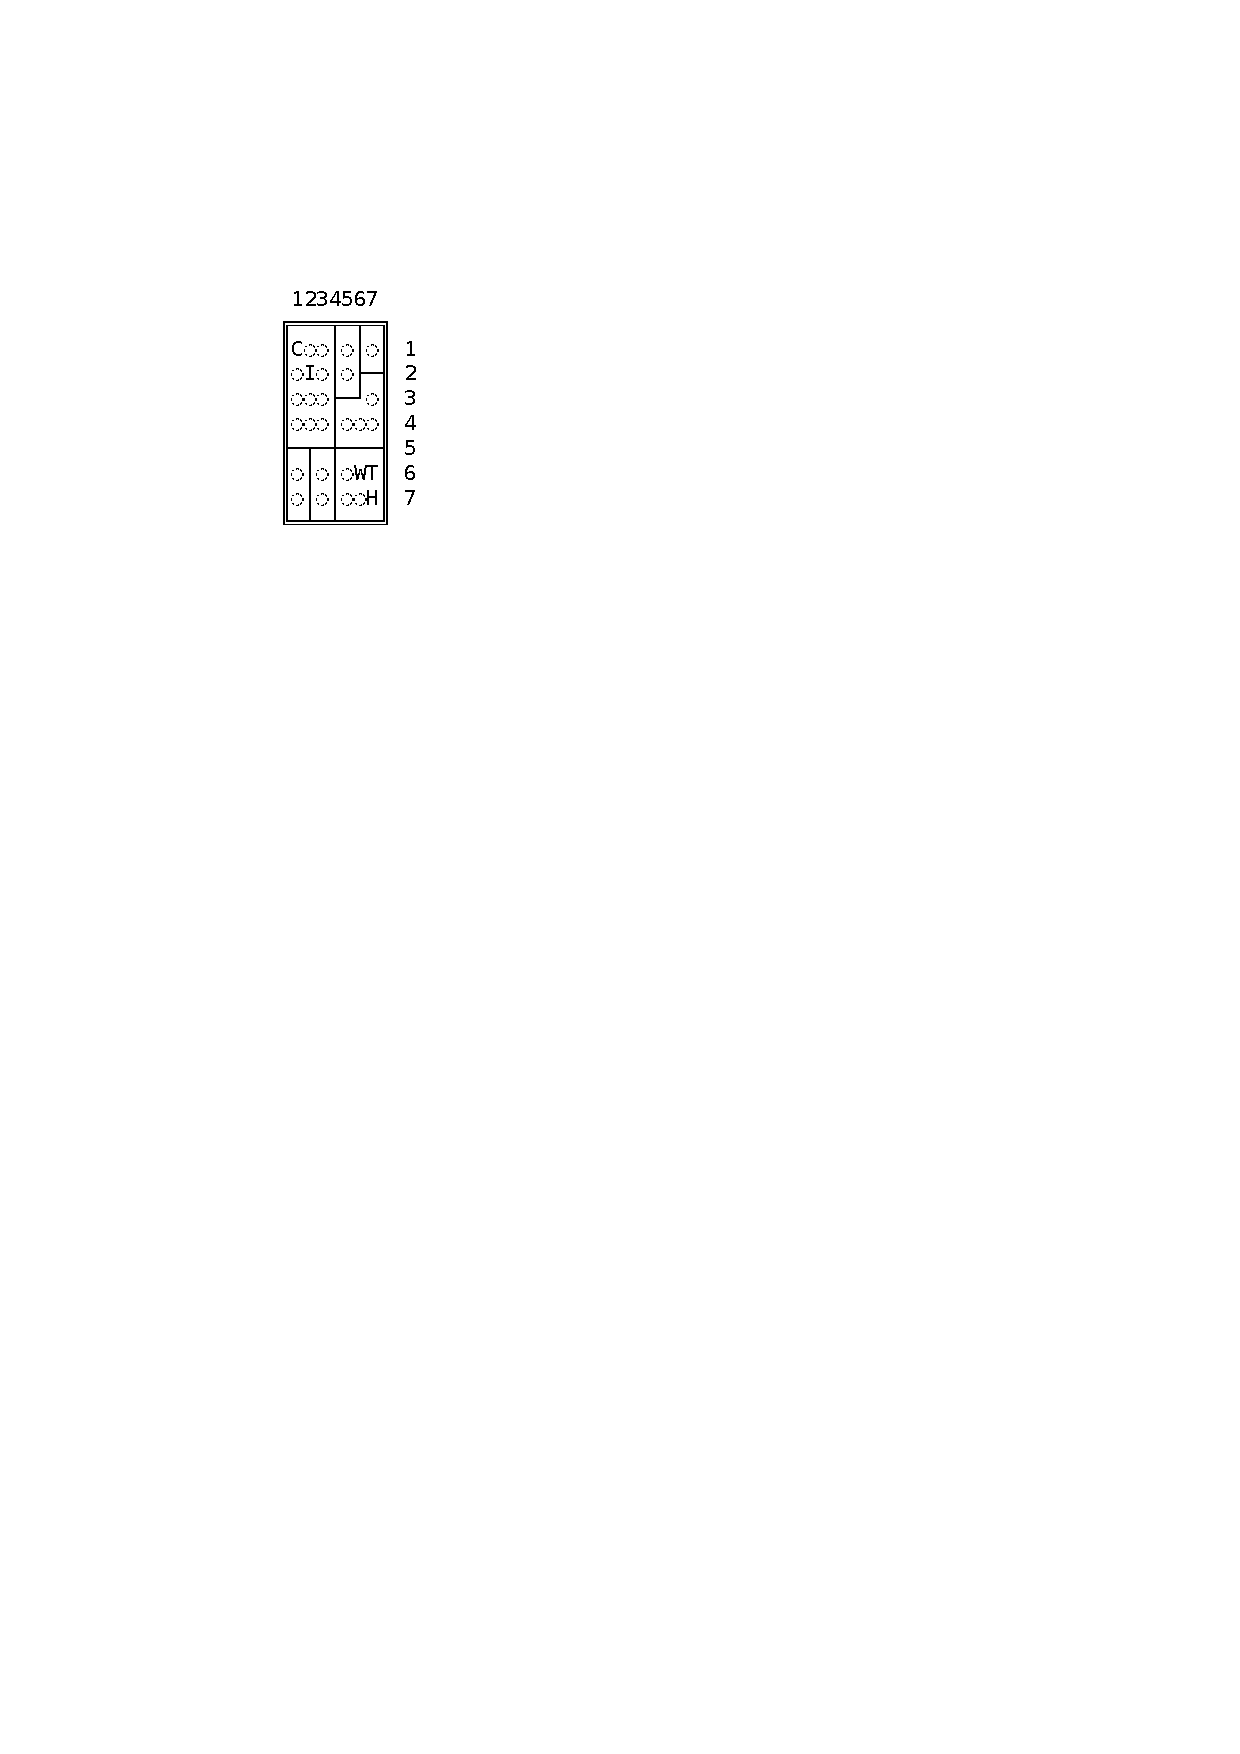
\includegraphics[height=60pt]{clean_up/grid_1_min.pdf}\\
                \raggedright
                \texttt{Please send a message to the other player to start the game!}
            }
        }
    }
    & \\

\theutterance \stepcounter{utterance}  
    & \multicolumn{4}{p{0.6\linewidth}}{
        \cellcolor[rgb]{0.561,0.737,0.561}{
            \makecell[{{p{\linewidth}}}]{
                \texttt{\tiny{[P1$\rangle$GM]}}
                \texttt{SAY: Hi! Let's coordinate our moves. [...]}
            }
        }
    }
    & & \\

\theutterance \stepcounter{utterance}  
    & & \multicolumn{4}{p{0.6\linewidth}}{
        \cellcolor[rgb]{0.9,0.9,0.9}{
            \makecell[{{p{\linewidth}}}]{
                \texttt{\tiny{[GM$\rangle$P2]}}
                \centering{<GAME DESCRIPTION>}\\
                \centering
                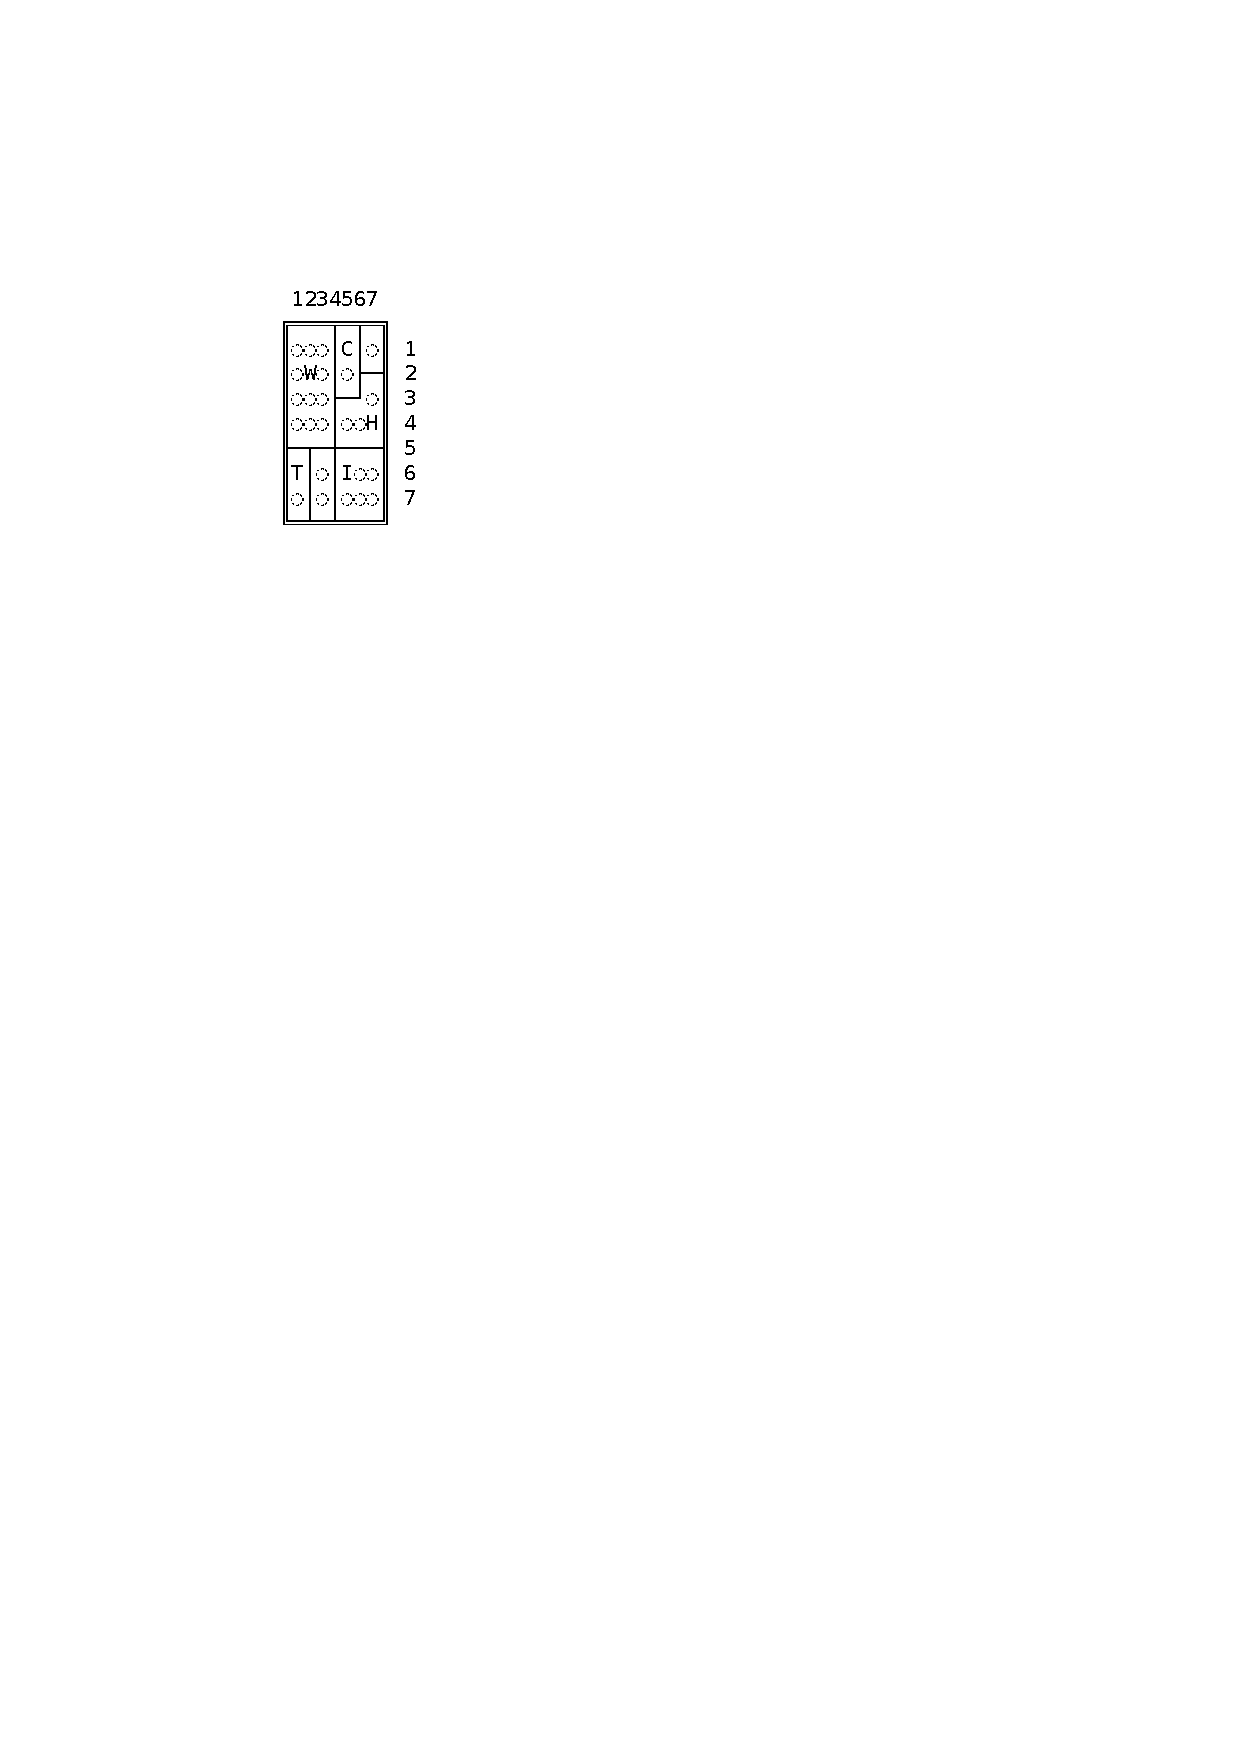
\includegraphics[height=60pt]{clean_up/grid_2_min.pdf}\\
                \raggedright
                \texttt{The other player started the game by sending this message:} \\
                \centering{<MESSAGE>}\\
                \raggedright
                \texttt{What is your first command?}
            }
        }
    }
    & \\

& \multicolumn{6}{c}{
\vdots
} \\

\theutterance \stepcounter{utterance}  
    & & & \multicolumn{4}{p{0.6\linewidth}}{
        \cellcolor[rgb]{0.373,0.62,0.627}{
            \makecell[{{p{\linewidth}}}]{
                \texttt{\tiny{[GM$\langle$P2]}}
                \texttt{MOVE: C, (1,1)} \\
            }
        }
    } \\

\theutterance \stepcounter{utterance}  
    & & \multicolumn{4}{p{0.6\linewidth}}{
        \cellcolor[rgb]{0.9,0.9,0.9}{
            \makecell[{{p{\linewidth}}}]{
                \texttt{\tiny{[P1$\langle$GM]}}
                Your message has been relayed to the other player.\\
                \centering <GAME STATE> \\
                \raggedright
                \texttt{The other player moved an object on their grid. \\What is your next command?}
            }
        }
    }
    & \\
    
\theutterance \stepcounter{utterance}  
    & \multicolumn{4}{p{0.6\linewidth}}{
        \cellcolor[rgb]{0.561,0.737,0.561}{
            \makecell[{{p{\linewidth}}}]{
                \texttt{\tiny{[P1$\rangle$GM]}}
                \texttt{MOVE: I, (5,6)}
            }
        }
    }
    & & \\

& \multicolumn{6}{c}{
    \vdots
} \\
\theutterance \stepcounter{utterance}  
    & & & \multicolumn{4}{p{0.6\linewidth}}{
        \cellcolor[rgb]{0.373,0.62,0.627}{
            \makecell[{{p{\linewidth}}}]{
                \texttt{\tiny{[GM$\langle$P2]}}
                \texttt{SAY: I think our grids are aligned now, finished?} \\
            }
        }
    } \\
\theutterance \stepcounter{utterance}  
    & \multicolumn{4}{p{0.6\linewidth}}{
        \cellcolor[rgb]{0.561,0.737,0.561}{
            \makecell[{{p{\linewidth}}}]{
                \texttt{\tiny{[P1$\rangle$GM]}}
                \texttt{SAY: finished!}
            }
        }
    }
    & & \\
\end{supertabular}
    \caption{Condensed example dialogue from Clean Up. The task is to negotiate a common goal configuration for a number of objects randomly placed on each player`s grid, and move them accordingly. Finally, both players have to agree the goal is reached to end the game. \kr{expand first P1 message}}
    % \vspace*{-.8cm}
    \label{fig:clean_up_example}
\end{figure}

\paragraph{Difficulty Levels and Instances}\label{sec:clean_up_difficulty_levels}  All grids have the same size ($7\times7$), and contain obstacles in form of horizontal and vertical lines, branches, crossings, and corners cf.~\cref{fig:clean_up_example}. They are generated using an ASP encoding to ensure all lines are continuous. We control difficulty along two dimensions: number of empty cells and number of objects.

More empty cells means it's less likely that players try to place objects in occupied cells. Of the 49 total cells, $34$ or $69.4\%$ of cells are empty on the \textit{easy} level, $29$ or $59.2\%$ on \textit{medium}, and $24$ or $49.0\%$ on \textit{hard} (cf.~\cref{clean_up:grid_examples} in \cref{clean_up_exp_setup} for example grids). For each level, we sample three grids, and then place $3$, $5$, or $7$ objects on them, making for $27$ experiments in total.

\paragraph{Game Mechanics} The game is turn based, and the maximum number of rounds is fixed to $4 \times n_{obj}$ (where $n_{obj}$ is the object count). Players can collectively accumulate $2 \times n_{obj} + 2$ penalties.

Initially, P1 (Player~1) is provided with a game description including round and penalty limit and their respective grid, following which they have to send a message to P2 (Player~2). P2 receives the same prompt and P1's message (see~\cref{fig:clean_up_prompt_templates} in \cref{clean_up:prompts} for the full prompt). In each turn, a player can either send a message to their counterpart or move an object on their grid.

Each following turn starts with a message from the Game Master consisting of three parts: (1) feedback on the last turn, i.~e., either a notification that the message has been passed on or the updated grid if they moved an object; (2) information on the game state, i.~e., current and maximum penalties and rounds, and (3) either the other player's message or a notification that they moved an object. 

If a player does not follow the format, tries to move an object to a non-empty space or outside the grid bounds, or tries to move an object that doesn't exist, they receive a penalty and are re-prompted with information on the nature of their mistake. See \cref{fig:clean_up_intermittent_prompts} in \cref{clean_up:prompts} for the full new turn and penalty messages.

The game ends if (1) both players agree to end it, (2) round limit is exceeded, or (3) penalty limit is exceeded.

\paragraph{Evaluation Metrics} A game counts as failure and is not scored if the penalty limit is exceeded. The Quality Score $\mathbf{QS}$ is calculated as follows:
$$\mathbf{QS} = \mathbf{DS} \cdot \mathbf{PS} \cdot 100; \ \mathbf{QS} \in [0, 100]$$

\textbf{Distance Score} $\mathbf{DS} \in [0,1]$ is calculated from three components, each representing the sum of Euclidean distances for all identical objects on both grids: the Initial Distance Sum $\mathbf{I}$ at the start of the game, the Final Distance Sum $\mathbf{F}$ at the end of the game, and the Expected Distance Sum $\mathbb{E}$ that approximates the distances for randomly placed objects (see \cref{clean_up:scoring} for details). The Expected Distance Score $ES$ and Distance Reduction Score $RS$, quantifying how close the players came to the goal of perfect alignment of all objects, are calculated as follows:
\begin{align*}
ES = \max \left\{0,1 - \frac{\mathbf{F}}{\mathbb{E}} \right\}; \
RS = \max \left\{0,1 - \frac{\mathbf{F}}{\mathbf{I}} \right\}
\end{align*}
$\mathbf{DS}$ is then either $0$ if final placement is worse than random, or calculated as the mean of both scores:
\begin{align*}
\mathbf{DS} &= \begin{cases}
\frac{ES+RS}{2} & if \quad ES > 0 \\
0 & otherwise
\end{cases}
\end{align*}

\textbf{Penalty Score} $\mathbf{PS} \in [0.5,1]$ is calculated from the penalty count $P$ normalized against max. penalties $P_m$ as follows:
$$\mathbf{PS} = \frac{P_m}{P-2P_m}+1.5$$
We chose the hyperbolic function because it is lenient for low $P$ and harsher for $P$ close to $P_m$.